\documentclass[12pt]{report}

\usepackage{amssymb, fullpage, amsmath, esint}
\usepackage{graphicx}

\newtheorem{problem}{Problem}

\newenvironment{solution}[1][\it{Solution}]{\textbf{#1. } }{$\square$}

\graphicspath{ {./} }

\allowdisplaybreaks

\pagestyle{empty}

\def\Z{{\mathbb Z}}
\def\Q{{\mathbb Q}}
\def\C{{\mathbb C}}
\def\R{{\mathbb R}}
\def\N{{\mathbb N}}
\def\eps{{\epsilon}}
\def\O{{\mathcal{O}}}
\newcommand{\floor}[1]{{\left\lfloor#1\right\rfloor}} % Floor function
\newcommand{\ceil}[1]{{\left\lceil#1\right\rceil}} % Ceiling function
\newcommand{\paren}[1]{{\left(#1\right)}} % Parentheses ()
\newcommand{\brac}[1]{{\left\{#1\right\}}} % Curly braces {}
\newcommand{\braces}[1]{{\left[#1\right]}} % Braces []
\newcommand{\abrac}[1]{{\left\langle#1\right\rangle}} % Angle Braces <>
\newcommand{\abs}[1]{{\left|#1\right|}} % Absolute value
\newcommand{\norm}[1]{{\left\|#1\right\|}} % Norm
\newcommand{\eval}[2]{\right|_{#1}^{#2}} % Evaluate

\newcommand{\pp}[2]{\frac{\partial #1}{\partial #2}} % Partial of 1 wrt 2
\newcommand{\ppn}[3]{\frac{\partial^{#1} #2}{\partial #3^{#1}}} % nth Partial of 1 wrt 2
\newcommand{\dd}[2]{\frac{\mathrm{d} #1}{\mathrm{d} #2}} % Partial of 1 wrt 2
\newcommand{\ddn}[3]{\frac{\mathrm{d}^{#1} #2}{\mathrm{d} #3^{#1}}} % nth Partial of 1 wrt 2

\def\ointcc{{\ointctrclockwise}} %counter clockwise contour integral
\def\ointc{{\ointclockwise}} %clockwise contour integral

%dash integral 
\def\Xint#1{\mathchoice
   {\XXint\displaystyle\textstyle{#1}}%
   {\XXint\textstyle\scriptstyle{#1}}%
   {\XXint\scriptstyle\scriptscriptstyle{#1}}%
   {\XXint\scriptscriptstyle\scriptscriptstyle{#1}}%
   \!\int}
\def\XXint#1#2#3{{\setbox0=\hbox{$#1{#2#3}{\int}$}
     \vcenter{\hbox{$#2#3$}}\kern-.5\wd0}}
\def\ddashint{\Xint=}
\def\dashint{\Xint-}


\begin{document}

\large

\begin{center}
 Math 584 Homework 7\\
 Due Soon\\
 By Marvyn Bailly\\
\end{center}

\normalsize

\hrule

%---------------%
%---Problem 1---%
%---------------%

%--status--$

\begin{problem}
    Let
    \[
    A = \left[ \begin{array}{cccc} 0 & 1 & 0 & 0 \\ 0 & 0 & 1 & 0 \\ 0 & 0 & 0 & 1 \\
    0 & 0 & 0 & 0 \end{array} \right] ,~~~
    A_{\epsilon} = \left[ \begin{array}{cccc} 0 & 1 & 0 & 0 \\ 0 & 0 & 1 & 0 \\
    0 & 0 & 0 & 1 \\ \epsilon & 0 & 0 & 0 \end{array} \right] ,~~\epsilon > 0.
    \]
    What are the eigenvalues of $A$ and of $A_{\epsilon}$?  Would you say that the problem of
    computing the eigenvalues of a matrix $A$ of this form is well-conditioned or ill-conditioned?
    Explain your answer.
\end{problem}

\begin{solution}
    \noindent
    Let
    \[
    A = \left[ \begin{array}{cccc} 0 & 1 & 0 & 0 \\ 0 & 0 & 1 & 0 \\ 0 & 0 & 0 & 1 \\
    0 & 0 & 0 & 0 \end{array} \right] ,~~~
    A_{\epsilon} = \left[ \begin{array}{cccc} 0 & 1 & 0 & 0 \\ 0 & 0 & 1 & 0 \\
    0 & 0 & 0 & 1 \\ \epsilon & 0 & 0 & 0 \end{array} \right] ,~~\epsilon > 0.
    \]
    To find the eigenvalues of $A$ observe that the characteristic polynomial is given by 
    \[ 
        \lambda^4 = 0,
    \]
    So all the eigenvalues of $A$ are $0$. The characteristic polynomial of $A_\eps$ is given by
    \[ 
        \lambda^4 = \epsilon
    \]
    so the eigenvalues of $A$ are the $4$th roots of $\epsilon$,
    \[ 
        \eps^{1/4}, -\eps^{1/4}, -i\eps^{1/4}, i\eps^{1/4}.
    \]
    Computing the eigenvalues of $A_\eps$ is is ill conditioned because a change in magnitude in $\eps$ will largely effect the eigenvalues of $A$. For example, if $\eps$ is perturbed by a very small amount, let's say $10^{-12}$, then the eigenvalue corresponding to $\eps^{1/4}$ will change by a factor of $10^{-4}$.



\end{solution}

%----------------------------------------------------------------------------------------------------%
%\vskip 20pt
\newpage

%---------------%
%---Problem 2---%
%---------------%

%--status--$

\begin{problem}
    p.~218, Exercise 28.1.
\end{problem}

\begin{solution}
    
    Let $A$ be an orthogonal matrix. Then when applying the unshifted QR algorithm to $A$, since $A$ is already orthogonal $R$ is just the identity matrix. Thus we have that $A=AR^{-1} = AI = A$. Thus we do not experience the behavior described in Theorem 28.4 of $A^{(k)}$ as $k \to \infty$. This makes sense since $A$ is orthogonal, the eigenvalues of $A$ must have magnitude $1$ and therefore we do not meet the requirement of Theorem 28.4 which says that each eigenvalue must be strictly greater than the next. 
\end{solution}

%----------------------------------------------------------------------------------------------------%
%\vskip 20pt
\newpage

%---------------%
%---Problem 3---%
%---------------%

%--status--$

\begin{problem}

    \noindent
    \begin{enumerate}
        \item
        Describe an $O( k^2 )$ algorithm based on QR factorization by Givens rotations 
        for solving the $k+1$ by $k$ upper Hessenberg least squares problem
        \[
        H_{k+1,k} y \approx \| r_0 \| \xi_1 ,
        \]
        that arises in the GMRES algorithm.
        \item
        Show how the operation count can be reduced to $O(k)$ if the problems at steps
        $1$ through $k-1$ have already been solved.
        [A general description is given at the bottom of p.~3 and top of p.~4 of the notes
        on Krylov Space Methods, but fill in the details.] 
        \end{enumerate}
        
\end{problem}

\begin{solution}
    
    \begin{enumerate}
        \item 
        We begin by decomposing $H_{k+1,k}$ using QR factorization to get
        \[ 
            Q_{k+1,k_1}H_{k_1,k} = R_{k+1,k} = \begin{pmatrix}
                R_{k,k}\\0
            \end{pmatrix}.
        \]
        Now notice that updating $H_{k+1,k}$ to $H_{k+2,k+1}$ can be done by
        \[ 
            H_{k+2,k+1} = \begin{pmatrix}
                H_{k+1,k} & h_{k+1}\\
                0 & k_{k+3,k+2}
            \end{pmatrix}.
        \]
        Thus when multiplying $Q_{k+1,k+1}$ by $H_{k+2,k+1}$ we get
        \[ 
            Q_{k+2,k+2}H_{k+2,k+1} = \begin{pmatrix}
                Q_{k+1,k+1} & 0 \\
                0 & 1
            \end{pmatrix} H_{k+2,k+1} = \begin{pmatrix}
                R_{k,k} & r_{k+1}\\
                0 & p\\
                0 & q
            \end{pmatrix},
        \]
        which is almost upper triangle. We can utilize Given rotations to get $q = 0$ with the matrix
        \[ 
            G_{k+2,k+2} = \begin{pmatrix}
                I_{k,k} & 0 & 0\\
                0 & c_k & s_k\\
                0 & -s_k & c_k
            \end{pmatrix}
        \]
        where $c_k = p/(p^2 + q^2)$ and $s_k = q/(p^2 + q^2).$ Then let's multiply $Q_{k+2,k+2}$ by the Givens matrix to get
        \[
            Q_{k+2,k+2} = G_{k+2,k_2}\begin{pmatrix}
                Q_{k+1,k+1} & 0 \\
                0 & 1
            \end{pmatrix}.
        \]
        Thus we have that
        \[ 
            Q_{k+2,k+2}H_{k+2,k+1} = \begin{pmatrix}
                R_{k,k} & r_{k+1}\\
                0 & \sqrt{p^2 + q^2}\\
                0 & 0
            \end{pmatrix},
        \]
        which is indeed upper triangle. This means that we preform $O(k^2)$ operation because we have to preform $k$ matrix multiplications. The upper triangle matrix can now be used to solve the least squares problem and minimize $y$. 

        \item
        If the problem has been solved at steps $1$ through $k-1$, then at the $k$th step, we only need to apply one more given rotation to zero the last entry of the last column of $H_{k+1,k}$ since we have saved all the previous given rotations. This final given rotation will only effect the last column and thus there will only be $0(k)$ cost at this step.

    \end{enumerate}
\end{solution}

%----------------------------------------------------------------------------------------------------%
%\vskip 20pt
\newpage

%---------------%
%---Problem 4---%
%---------------%

%--status--$

\begin{problem}
    Show that if $A$ is Hermitian and positive definite, the `$A$-norm' of a vector, 
defined as
\[
\| v \|_A := ( v^{*} A v )^{1/2}
\]
is, indeed, a norm.
\end{problem}

\begin{solution}
    
    Let $A$ be a Hermitian positive definite matrix. Then by definition of $A$ we have that
    \[ 
        v^*Av > 0 ~~\forall v \neq 0 ~~ \text{and} ~~ A = LL^*,
    \]
    where $LL^*$ is the Cholesky decomposition. We define the $A$-norm as
    \[
    \| v \|_A := ( v^{*} A v )^{1/2},
    \] 
    and wish to verify that it is a norm. Firstly observe that
    \[ 
        \| A \|_A = (v^* A v)^{1/2} > 0,
    \]
    since $v^*Av > 0$ where equality is achieved only if $v=0$. Next let $\alpha$ be some constant, then  
    \begin{align*}
        \| \alpha v \|_A &= \paren{(\alpha v)^* A (\alpha v)}^{1/2}\\
        &=\paren{v^*\alpha^*A\alpha v}^{1/2}\\ 
        &= (\alpha^*\alpha)^{1/2}(v^*Av)^{1/2}\\
        &= |\alpha|\|v\|_A.
    \end{align*}
    Lastly note that we can use the Cholesky decomposition to rewrite the $A$-norm as
    \[ 
        \|v\|_A = (v^*Av)^{1/2} = (v^*LL^*v)^{1/2} = ((L^*v)^*(L^*v))^{1/2} = \|L^*v\|_2
    \]
    Then we can show the triangle inequality by observing
    \begin{align*}
        \|u + v\|_A &= ((u+v)^*A(u+v))^{1/2}\\
        &= ((u^*+v^*)LL^*(u+v))^{1/2}\\
        &= ((L^*(u+v))^*(L^*(u+v)))^{1/2}\\
        &=\| L^*(u+v) \|\\
        &= \| L^*u + L^*v\|_2\\
        &\leq \|L^*u\|_2 + \|L^*v\|_2\\
        &= \|u\|_A + \|v\|_A.
    \end{align*}
    Thus we have verified that the $A$-norm is a norm. 
\end{solution}

%----------------------------------------------------------------------------------------------------%
%\vskip 20pt
\newpage

%---------------%
%---Problem 5---%
%---------------%

%--status--$

\begin{problem}

    \noindent
    \begin{enumerate}
        \item
        The CG algorithm is applied to a Hermitian positive definite linear system $Ax=b$.
        The $A$-norm of the error in the initial guess is $1$, and the $A$-norm of the 
        error at step $10$ is $2 \times 2^{-10}$.  Based on this information alone, what
        bound can you give on $\kappa (A)$?  Explain how you get your answer.
        \item
        Suppose a positive definite matrix has a small, well-separated eigenvalue:
        $\lambda_1 << \lambda_2 \leq \ldots \leq \lambda_m$ (that is, $\lambda_1 / \lambda_2 << 1$).
        Derive an error bound for CG using the maximum value of a polynomial that is the
        product of a linear factor $( \lambda_1 - z)/ \lambda_1$ and a $(k-1)$st degree
        Chebyshev polynomial on the interval $[ \lambda_2 , \lambda_m ]$.  Comparing your
        result with inequality (10) in the notes on Krylov Space Methods, would you say that
        it is more advantageous to have a small, well-separated eigenvalue or a large,
        well-separated eigenvalue as in (10)?
    \end{enumerate}
\end{problem}

\begin{solution}
    
    \begin{enumerate}
        \item 
        Consider the CG algorithm applied to a Hermitian positive definite linear system $Ax = b$. We have that the error in the initial guess is $\|e_0\|_A = 1$ and that the error at step $10$ is $\| e^{\text{CG}}_{10} \|_{A} = 2 \times 2^{-10}$. By Theorem 1 in the Krylov notes we have that
        \[ 
            \frac{\|e^{\text{CG}}_{k} \|_{A}}{\|e_0\|_A} \leq 2\paren{\frac{\sqrt{\kappa} - 1}{\sqrt{\kappa} + 1}}^k,
        \]
        where $\kappa = \lambda_{\text{max}} / \lambda_{\text{min}}$. Note that
        \[ \kappa(A) = \frac{\sigma_{\text{max}}}{\sigma_{\text{min}}} = \frac{|\lambda_{\text{max}}|}{|\lambda_{\text{min}}|} = \frac{\lambda_{\text{max}}}{\lambda_{\text{min}}} = \kappa.\] 
        Plugging in our values and solving for $\kappa$ we get
        \begin{align*}
            2\times 2^{-10} \leq 2\paren{\frac{\sqrt{\kappa} - 1}{\sqrt{\kappa} + 1}}^{10} \implies
            \frac{1}{2} \leq \frac{\sqrt{\kappa} - 1}{\sqrt{\kappa} + 1} \implies
            -\sqrt{\kappa} \leq -3 \implies
            \kappa \geq 9.
        \end{align*}
        Thus we have bounded $\kappa(A) \geq 9$.
        \item 
        Suppose a positive definite matrix has a small, well-separated eigenvalue:
        $\lambda_1 << \lambda_2 \leq \ldots \leq \lambda_m$ (that is, $\lambda_1 / \lambda_2 << 1$). To derive an error bound consider the product of $(\lambda_1 - z)/\lambda_1$ and a $(k-1)$st degree Chebyshev polynomial on the interval $[\lambda_2,\lambda_m].$ That is,
        \[
            p_k(z)=\paren{\frac{\lambda_1 - z}{\lambda_1}} \paren{T_{k-1}\paren{\frac{2z - \lambda_m -\lambda_2}{\lambda_m - \lambda_2}} \left/T_{k-1}\paren{\frac{-\lambda_m - \lambda_2}{\lambda_m - \lambda_2}}\right.}.
        \]
        Then the first term is bounded by $\abs{\frac{\lambda_1 - \lambda_m}{\lambda_1}}$ and the second term is bounded by $2\paren{\frac{\sqrt{\kappa_m} - 1}{\sqrt{\kappa_m} + 1}}^{k-1}$ where $\kappa_m = \lambda_m/\lambda_2$ by the Theorem 1 in the Krylov notes. Then the error bound is given by 
        \[ 
            \frac{\|e^{\text{CG}}_{k} \|_{A}}{\|e_0\|_A} \leq 2\abs{\frac{\lambda_1 - \lambda_m}{\lambda_1}}\paren{\frac{\sqrt{\kappa_m} - 1}{\sqrt{\kappa_m} + 1}}^{k-1}.
        \]
        Comparing this bound with the inequality (10) in the Krylov notes, we can see that it is more advantageous to have a large, well-separated eigenvalue as in (10).
    \end{enumerate}
\end{solution}

%----------------------------------------------------------------------------------------------------%
%\vskip 20pt
\newpage

%---------------%
%---Problem 6---%
%---------------%

%--status--$

\begin{problem}
    You can set up a sparse matrix defining a finite difference approximation for
    Laplace's equation on an L-shaped domain in Matlab by typing
    \verb+A = delsq(numgrid('L',500))+.  Matlab stores just the nonzero
    entries of the matrix along with their row numbers and column numbers.
    You can see where $A$ has nonzeros by typing \verb+spy(A)+,
    and you can see the size of $A$ by typing \verb+[m,m] = size(A)+.
    Set a random vector $b$ of length $m$ and use unpreconditioned CG
    to solve $Ax=b$ for $x$.  You may use \verb+pcg+ in Matlab.  Type:
    \begin{verbatim}
    tic, [x,flag,relres,iter,resvec] = pcg(A,b,tol,m), toc
    \end{verbatim}
    where \verb+tol+ is a desired tolerance, say, $1.0e-8$.  
    This will time the routine and print out the time spent.
    The array \verb+resvec+ returned by \verb+pcg+ contains the 2-norm of the 
    residual at each step of the CG algorithm.  Plot the entries of \verb+resvec+ 
    vs. iteration number using a \verb+semilogy+ plot so that small values of 
    the residual norm can be distinguished.  Now try solving $Ax=b$ using CG 
    with an incomplete Cholesky decomposition as a preconditioner.  You can 
    get the incomplete Cholesky decomposition of $A$ by typing \verb+L = ichol(A)+.  
    You can then send this to \verb+pcg+ by typing
    \begin{verbatim}
    tic, [x,flag,relres,iter,resvecic] = pcg(A,b,tol,m,L,L'); toc
    \end{verbatim}
    Plot the residual norms at each step of the preconditioned algorithm on
    the same plot as those of the unpreconditioned algorithm.  Turn in your
    plot of residual norms, with the different convergence curves labeled.  
    Try a few different runs and report on which algorithm is usually faster.
\end{problem}

\begin{solution}
    
    I wrote the following MatLab code for this problem
    \begin{verbatim}
        A = delsq(numgrid('L',500));
        [m,m] = size(A);
        b = rand(m,1);
        tol = 1.0 * 10^(-8);
        tic, 
        [x,flag,relres,iter,resvec] = pcg(A,b,tol,m); 
        toc

        semilogy(0:iter,resvec)
        hold on

        L = ichol(A);
        tic,
        [x,flag,relres,iter,resvecic] = pcg(A,b,tol,m,L,L');
        toc

        semilogy(0:iter,resvecic)
        hold off

        legend("unpreconditioned","preconditioned");
    \end{verbatim}
    which gives the following plot
    \begin{center}
        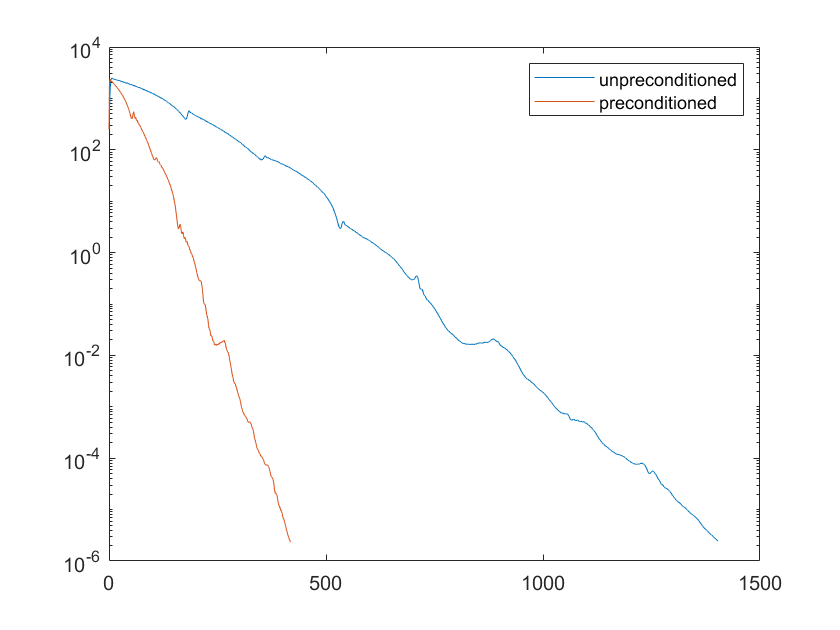
\includegraphics[width=.6\textwidth]{plots/6-1.png}
    \end{center}
    and the following output
    \begin{verbatim}
        >> hw7q6
            Elapsed time is 8.819515 seconds.
            Elapsed time is 6.576605 seconds.
        >> hw7q6
            Elapsed time is 8.947682 seconds.
            Elapsed time is 6.400742 seconds.
    \end{verbatim}
    Running the algorithm a few times and observing the time results of each algorithm shows that the preconditioned algorithm runs faster and takes less iterations than the unpreconditioned.
\end{solution}

%----------------------------------------------------------------------------------------------------%
%\vskip 20pt
\newpage


\end{document}